% =====================================================================
%  Chapter 2 — Five Handles on the Missing Mass
% =====================================================================

\chapter{Five Handles on the Missing Mass}
\label{ch:handles}

A single measurement of something invisible is an interpretation. Five
measurements that agree are a fact. The reason the density of dark matter is
believed is that five physically unrelated routes to it converge, using
different instruments, different physics and different sets of assumptions.

\section{First handle: rotation curves}The first handle was turned in 1939, when Horace Babcock reported
that the spiral NGC~3190 rotated too fast at large radii for its visible
mass \idx{Babcock}. Vera Rubin and Kent Ford established the phenomenon
systematically a generation later, and their 1970 paper remains the standard
citation for it \idx{Rubin and Ford}. The radial velocity of stars in a
spiral galaxy stays flat instead of falling as $v \sim r^{-1/2}$, and the
only way to keep the outer stars bound is to supply mass that emits no
light.

The modern form of the argument is a pressure profile: gas in the disc
dissociates at a characteristic radius, and the observed rotation curve
divided by that radius measures the total enclosed mass. The result is a
mass-to-light ratio that rises with radius in every spiral examined, and
rises to values of ten to one hundred at the outskirts where the visible
matter has run out.

Rotation curves are the strongest handle in the sense that they cover the
largest number of objects, and the weakest in the sense that they are most
sensitive to the baryonic processes --- feedback, star formation history,
gas geometry --- that models of galaxy formation must reproduce. They
constrain the dark matter halo, not the dark matter particle.

\section{Second handle: cluster dynamics}Galaxy clusters supply the mass in a way that does not depend on
gas dynamics at all. The virial theorem applied to a cluster's member
galaxies gives a total mass, and X-ray observations of the intracluster gas
give a baryonic mass. The two disagree by a factor of five to eight in
favour of more mass.

What makes this handle powerful is the independent confirmation from a
different gas: the cluster's gravitational field is also mapped by the
temperature of the X-ray-emitting gas through X-ray hydrostatic mass
estimates, and by the distribution of galaxy velocities through dynamical
mass estimates. Where the baryons are measured in three different ways, they
are consistently too light to hold the clusters together.

\section{Third handle: gravitational lensing}Light bending measures mass without reference to the light.
Weak lensing --- the slight, statistical distortion of background galaxies
by foreground mass --- maps the mass distribution in clusters and in the
cosmic web, and strong lensing --- multiple images of a background source ---
provides a direct distance measurement that does not rely on any luminosity
model at all. The Bullet Cluster in Chapter~\ref{ch:bullet} is the extreme
case of strong lensing.

The cosmological leverage of weak lensing has been growing quickly, and by
2026 the combination of DESI's spectroscopic redshifts with DES and HSC
weak-lensing maps is a serious competitor to the CMB for structure
constraints. That is a development with consequences for Part~\ref{part:decision}:
if weak lensing can measure the growth of structure as well as the CMB can
measure its initial conditions, then some of the cosmological tension
discussed in Chapter~\ref{ch:tensions} becomes experimentally decidable
without leaving the galaxy survey.

\section{Fourth handle: the CMB acoustic peaks}Chapter~\ref{ch:budget} covered this handle in detail, because it is
the most precise. Its role here is structural: it is the only one of the
five that measures the density in the early universe and extrapolates, while
the other four measure it in the present universe and extrapolate back.
The agreement between early-universe extrapolation and late-universe
measurement is the reason the density is believed, and the systematic
disagreement between them --- visible in the tension between CMB-inferred
and locally-inferred values of $H_0$ --- is the reason the field is looking
for new physics in cosmology itself.

\section{Fifth handle: baryon acoustic oscillations}The last handle comes from the fossil of the sound waves in the
early universe, imprinted on the distribution of galaxies. The sound horizon
at recombination has a physical size, set by the photon-baryon fluid and the
expansion rate, and it leaves a characteristic ruler in the correlation
function of the galaxy distribution.

The ruler is measured two ways. In the radial direction, using the
correlation of galaxy pairs along the line of sight, it gives the distance
scale; in the transverse direction, the angle subtended by the ruler gives
the angular diameter distance. The ratio of the two is the Hubble parameter
at the redshifts in question, and it agrees well with the value inferred from
the CMB --- which is itself remarkable, because the two measurements use
different epochs, different instruments and different sets of assumptions.

DESI's second data release, covering more than 14 million galaxies over
seven redshift bins, is the most precise measurement of the ruler yet
made \idx{DESI Collaboration}. It is also the measurement that has opened the
most interesting tension in cosmology, which is the subject of
Chapter~\ref{ch:tensions}.

\begin{figure}[!htbp]
\centering
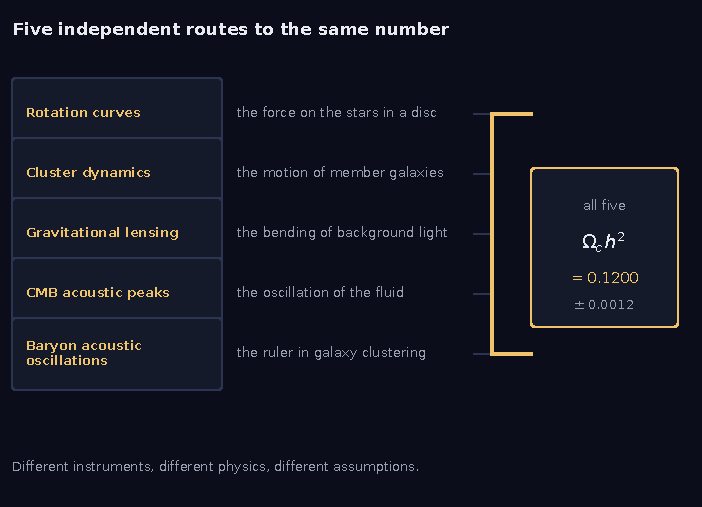
\includegraphics[width=\textwidth]{../figures/fig_handles.pdf}
\caption{The five handles on the missing mass. Each measures the same
quantity by a different physical route: rotation curves infer it from the
gravitational force on stars, cluster dynamics from the motion of member
galaxies, lensing from the bending of background light, the CMB acoustic
peaks from the oscillation of the photon-baryon fluid, and baryon acoustic
oscillations from the fossil ruler left in galaxy clustering.}
\label{fig:handles}
\end{figure}

\section{Why convergence is the argument}The five handles have different vulnerabilities, and that is the
point. Rotation curves could in principle be explained by atypical baryonic
feedback; cluster dynamics depends on understanding the intracluster gas;
lensing depends on the lensing source's redshift distribution and on
shear calibration; the acoustic peaks depend on the cosmological model
underlying the analysis; baryon acoustic oscillations depend on the galaxy
population being unbiased.

\begin{keytakeaways}
\item Five physically independent routes measure the same density: rotation
curves, cluster dynamics, gravitational lensing, CMB acoustic peaks, and
baryon acoustic oscillations.
\item Each handle has its own vulnerability, and no single handle's failure
would be fatal to the conclusion --- which is what makes the convergence the
argument rather than any one measurement.
\item Weak lensing combined with DESI spectroscopy is becoming competitive
with the CMB as a structure probe, which changes what a tension in cosmology
would mean.
\end{keytakeaways}
